\documentclass[a4paper,english,12pt]{article}
\usepackage{dsfont}
\usepackage{%
	amsfonts,%
	amsmath,%	
	amssymb,%
	amsthm,%
	algorithm,%
	babel,%
	bbm,%
	etex,%
	%biblatex,%
	caption,%
	centernot,%
	color,%
	dsfont,%
	enumerate,%
	epsfig,%
	epstopdf,%
	geometry,%
	graphicx,%
	hyperref,%
	latexsym,%
	mathtools,%
	multicol,%
	pgf,%
	pgfplots,%
	pgfplotstable,%
	pgfpages,%
	proof,%
	psfrag,%
	subfigure,%	
	tikz,%
	ulem,%
	url%
}	
\usepackage[noend]{algpseudocode}
\usepackage[mathscr]{eucal}
\usepgflibrary{shapes}
\usetikzlibrary{%
  	arrows,%
	backgrounds,%
	chains,%
	decorations.pathmorphing,% /pgf/decoration/random steps | erste Graphik
	decorations.text,%
	matrix,%
  	positioning,% wg. " of "
  	fit,%
	patterns,%
  	petri,%
	plotmarks,%
  	scopes,%
	shadows,%
  	shapes.misc,% wg. rounded rectangle
  	shapes.arrows,%
	shapes.callouts,%
  	shapes%
}

\theoremstyle{plain}
\newtheorem{thm}{Theorem}[section]
\newtheorem{lem}[thm]{Lemma}
\newtheorem{prop}[thm]{Proposition}
\newtheorem{cor}[thm]{Corollary}

\theoremstyle{definition}
\newtheorem{defn}[thm]{Definition}
\newtheorem{conj}[thm]{Conjecture}
\newtheorem{exmp}[thm]{Example}
\newtheorem{assum}[thm]{Assumptions}
\newtheorem{axiom}[thm]{Axiom}

\theoremstyle{remark}
\newtheorem{rem}{Remark}
\newtheorem{note}{Note}
\newtheorem{fact}{Fact}

\newcommand{\norm}[1]{\left\lVert#1\right\rVert}
\newcommand{\indep}{\!\perp\!\!\!\perp}
\DeclarePairedDelimiter\abs{\lvert}{\rvert}%
\newcommand\numberthis{\addtocounter{equation}{1}\tag{\theequation}}
\newcommand{\tr}{\operatorname{tr}}
\newcommand{\R}{\mathbb{R}}
\newcommand{\N}{\mathbb{N}}
\newcommand{\E}{\mathbb{E}}
\newcommand{\Z}{\mathbb{Z}}
\newcommand{\B}{\mathscr{B}}
\newcommand{\C}{\mathcal{C}}
\newcommand{\T}{\mathscr{T}}
\newcommand{\F}{\mathcal{F}}
\newcommand{\G}{\mathcal{G}}
%\newcommand{\ba}{\begin{align*}}
%\newcommand{\ea}{\end{align*}}
\DeclareMathOperator*{\argmax}{arg\,max}
\renewcommand{\qedsymbol}{$\blacksquare$}
\makeatletter
\def\BState{\State\hskip-\ALG@thistlm}
\makeatother

\makeatletter
\def\th@plain{%
  \thm@notefont{}% same as heading font
  \itshape % body font
}
\def\th@definition{%
  \thm@notefont{}% same as heading font
  \normalfont % body font
}
\makeatother
\date{}

%opening
\title{Lecture 4: Solved Problems}
\date{21 Jan 16}

\begin{document}
\maketitle
  
\section{Continued from the Lecture 3}
The following is the summary of Bayesian, Minimax and Neyman Pearson hypothesis testing:
\subsection{Bayesian Hypothesis Testing}
There are two possible hypotheses $H_{0}$ and $H_{1}$, corresponding to two possible probability distributions $P_{0}$ and $P_{1}$, respectively on the observation set $(\Gamma)$.This problem is written as
\begin{eqnarray}
H_{0}:Y\sim P_{0}\\\nonumber
H_{1}:Y\sim P_{1}
\end{eqnarray}
The decision rule $\delta$ as a function on $\Gamma$ is given by
\begin{eqnarray}
\delta(y)=\mathds{1}_{\{y\in\Gamma_{1}\}}
\end{eqnarray}
We define expected cost incurred by decision rule $\delta$ when hypothesis $H_{j}$ is true i.e.,
\begin{eqnarray}
R_{j}(\delta)= C_{1j}P_{j}(\Gamma_{1})+C_{0j}P_{j}(\Gamma_{0})
\end{eqnarray}
where $\Gamma_0$ is the rejection region $\Gamma_1$ is the  acceptance region.
The Bayes risk or the overall cost incurred by decision rule $\delta$ is given by
\begin{align}
r(\delta)&= \pi_{0}R_{0}(\delta)+\pi_{1}R_{1}(\delta)\nonumber\\
         &= \pi_{0}R_{0}(\delta)+(1-\pi_{0})R_{1}(\delta)
\end{align} 
where $\pi_{0}$ and $\pi_{1}$ are known as the priori probabilities of the two hypotheses $H_0~and~H_1$ respectively.
\par A commonly used cost assignment is the uniform cost given by
\begin{equation}
C_{ij}= 
		\begin{cases}
		0~~\mbox{if}~~i=j\\
		1~~\mbox{if}~~i\neq j\\
		\end{cases}
\end{equation}
Conditional risks are given~by
\begin{eqnarray}		
  R_{0}(\delta)=P_{0}(\Gamma_{1})\nonumber\\
  R_{1}(\delta)=P_{1}(\Gamma_{0})\nonumber     
\end{eqnarray}
\subsection{Minimax Hypothesis Testing}
The minimax rule is given by
\begin{equation}
\min_{\delta}\max({R_{0}(\delta),R_{1}(\delta)})
\end{equation}
Or equivalently
\begin{align}
\min_{\delta}\max_{0 \leq \pi_{0} \leq 1}r(\pi_{0},\delta)&= \max_{0 \leq \pi_{0} \leq 1}\min_{\delta}r(\pi_{0},\delta)\nonumber\\
														  &= \max_{0 \leq \pi_{0} \leq 1}V(\pi_{0})
\end{align}
where $V(\pi_{0})=\min_{\delta}r(\pi_{0},\delta)$ and the Minimax rule is achieved where $\pi_{0}$ is such that
\begin{equation} 
R_{0}(\delta_{\pi_{0}})=R_{1}(\delta_{\pi_{0}})
\end{equation}

\subsection{Neyman-Pearson Hypothesis Testing}
The design criterion for Neyman-Pearson hypothesis testing is 
\begin{eqnarray}
\max_{\delta}P_{D}(\delta)~subject~to~P_{F}(\delta)\leqslant\alpha
\end{eqnarray}
where $P_D(\delta)$ is the probability of correct detection and $P_F(\delta)$ which is the probability of false alarm and upper bounded by $\alpha$. The randomized decision rule is written as
\begin{eqnarray}
\tilde{\delta}(y)= \begin{cases} 1   ~~L(y)>\eta\\
                   \gamma(y)~~L(y)=\eta\\
                   0   ~~L(y)<\eta
                  \end{cases}\\
\therefore \tilde{\delta}(y)= \mathds{1}_{\{L(y)>y\}}+\gamma(y)\mathds{1}_{\{L(y)=y\}} \label{NP}               
\end{eqnarray}
where $\tilde{\delta}$ is the conditional probability with which we accept $H_1$ for a given observation $Y=y$, $L(y)=\frac{p_1(y)}{p_0(y)}$ is the likelihood function ant $\eta\geq0$ is certain threshold and $0\leq\gamma(y)\leq1$. with $\eta= \eta_0$ and $\gamma(y) = \gamma_0$ we have
\begin{align} 
\eta_{0}   &= \inf{\{\eta\in{\rm I\!R}:P_{0}\{L(y)>\eta\}\leqslant\alpha\}} \\
\gamma_{0} &= \frac{\alpha-P_{0}\{L(y)>\eta\}}{P_{0}\{L(y)=\eta\}}    
\end{align}
$P_0(L(y)>\eta)$ as a function of $\eta$ is shown in figure \ref{fig:Neyman1}. This can be interpreted as the \textit{complementary distribution function} (i.e. 1-distribution function) of the likelihood function and hence right continuous and may have discontinuity. From figure \ref{fig:Neyman1} it is clear that $0\leq\alpha-P_{0}\{L(y)>\eta\}\leq P_{0}\{L(y)=\eta\}$ and hence $0\leq\gamma_0\leq1$.
\begin{figure}[h]
\centering
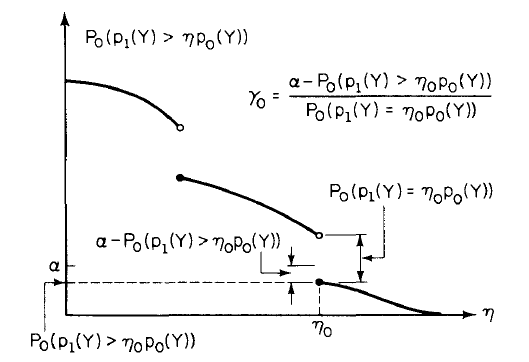
\includegraphics[width=0.6\linewidth]{Figures/Neyman}
\caption{Threshold and randomization for $\alpha$ level Neyman-Pearson test}
\label{fig:Neyman1}
\end{figure}
\begin{exmp}[Location testing with Gaussian error] 
Consider the following problem where we have a real-valued measurement (\textit{Y}), which is corrupted with Gaussian noise (n) having zero mean and standard deviation $\sigma$. Here the observation space is real line $\Gamma=\rm I\!R$.
\begin{equation}
Y=X+n
\end{equation}
where $X\in{\{\mu_{0},\mu_{1}\}}$ is the original signal and $n\in{\mathcal{N}(0,\sigma^{2})}$. In this example the Null Hypothesis $(H_{0})$ indicates transmission of Signal with mean $\mu_{0}$ and Alternative Hypothesis $(H_{1})$ indicates transmission of Signal with mean $\mu_{1}$. Without the loss of generality let us assume $\mu_{1}>\mu_{0}$.
\begin{eqnarray}
{H_0} :Y \sim \mathcal{N} \left( \mu _0, \sigma^2\right) \\
{H_1} :Y \sim \mathcal{N} \left( \mu _1, \sigma^2\right)
\end{eqnarray}
where $\mathcal{N}( \mu _0, \sigma^2)$ is the Gaussian distribution with mean $\mu$ and variance $\sigma^{2}$. $\mathcal{N}(\mu _0, \sigma^2)$ random variable has the probability density function $Pr(X=x)=\frac{exp{\bigl(-\frac{(x-\mu)^{2}}{\sigma^{2}}\bigl)}}{\sqrt{2\pi}}$.
\\\\
\textbf{Bayesian Hypothesis testing}\\\\
 Now the likelihood function is given by 
\begin{align}
L(y)&=\frac{p_{1}(y)}{p_{0}(y)} \nonumber
	=\dfrac{\frac{1}{\sqrt{2\pi}}exp{\bigl(-\frac{(x-\mu_{0})^{2}}{\sigma^{2}}\bigr)}}{\frac{1}{\sqrt{2\pi}}exp{\bigl(-\frac{(x-\mu_{1})^{2}}{\sigma^{2}}\bigr)}}\nonumber\\
	&=exp\biggl(\frac{\mu_{1}-\mu_{0}}{\sigma^{2}}\bigl(y-\dfrac{\mu_{1}+\mu_{0}}{2}\bigr)\biggr)
\end{align}
The Bayes rule is given by 
\begin{equation}
\delta_{B}(y)=\mathds{1}_{\{ L(Y)>\tau\}}
\label{(eq:25)}
\end{equation}
Where $\tau$ is the appropriate threshold expressed in terms of prior probability of Null Hypothesis $\pi_{0}$ as $\tau=\frac{\pi_{0}}{1-\pi_{0}}$
Equivalently equation \ref{(eq:25)} can be written as comparing Y with another threshold $\tau'=L^{-1}(\tau)$ . Hence $\delta_{B}(y)=\mathds{1}_{\{ Y>\tau'\}}$
Where
\begin{equation}
\tau'=\frac{\mu_{0}+\mu_{1}}{2}+\frac{\sigma^{2}}{\mu_{0}-\mu_{1}}\log(\tau)\label{eq:28}
\end{equation}
For example, with uniform costs and equal priors we have $\tau=1$ and $\tau'=(\dfrac{\mu_{0} + \mu_{1}}{2})$. Thus, in this particular case, the Bayes rule compares the observation to the average of $\mu_{0}$ and $\mu_{1}$. If \textit{y} is greater than or equal to the average, we choose $H_{1}$; if \textit{y} is less than this average, we choose $H_{0}$. This test is illustrated in figure \ref{fig:locationtesting}.
\begin{figure}[h]
\centering
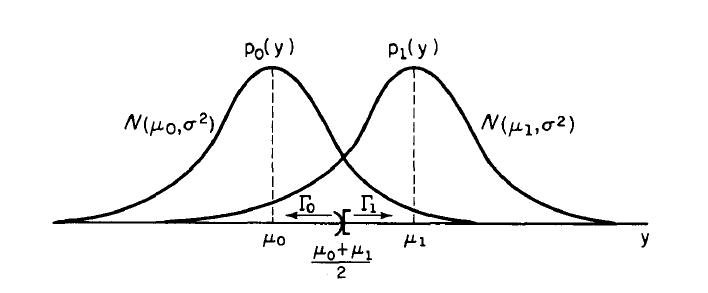
\includegraphics[width=0.75\linewidth]{Figures/Location_Gaussian}
\caption{Illustration of location testing with Gaussian error with uniform cost and equal prior}
\label{fig:locationtesting}
\end{figure}
We can write $P_j(\Gamma_1)~ for~j=0,1$ as follows.
\begin{align}
P_{j}(\Gamma_{1})&=\int\limits_{{\Gamma_1}}  {d{P_j}(y)}
				=\int\limits_{{\tau'}}^\infty  {d{P_j}(y)},~[since~ \Gamma_1=\{y\in{\rm I\!R}|y\geq\tau'\}]\nonumber\\
				&=\int\limits_{{\frac{\tau'-\mu_j}{\sigma}}}^\infty  {d{P}(\tau)}\nonumber\\
				&=1-\Phi\Bigl(\frac{\tau'-\mu_j}{\sigma}\Bigr)
				\end{align}
Now from equation \ref{eq:28} we can write the following
\begin{equation}
P_{j}(\Gamma_{1})= 
				  \begin{cases} 
				   1-\Phi\Bigl(\frac{\log(\tau)}{d}+\frac{d}{2}\Bigr) & \text{if }  j= 0 \\
				   1-\Phi\Bigl(\frac{\log(\tau)}{d}-\frac{d}{2}\Bigr) & \text{if }  j= 1
				  \end{cases}
\end{equation}
Where $d=\frac{\mu_{1}-\mu_{0}}{\sigma}$ is a simple version of \textit{signal-to-noise ratio(SNR)} and $\Phi$ denotes the cumulative distribution function of a $\mathcal{N}( 0, 1)$. Now the unconditional risk is the following
\begin{equation}
r\bigl(\pi_0,\delta_{\pi_{0}}\bigr)=\pi_0\biggl(1-\Phi\Bigl(\frac{\tau'-\mu_j}{\sigma^2}\Bigr)\biggr)+(1-\pi_0)\Phi\Bigl(\frac{\tau'-\mu_j}{\sigma^2}\Bigr)\label{eq:33}
\end{equation}
For equal prior \textit{e.i.} $\pi_0=\pi_1=\frac{1}{2}$ we have
\begin{align}
r\Bigl(\frac{1}{2},\delta_{\frac{1}{2}}\Bigr)&=\frac{1}{2}\biggl(1-\Phi\Bigl(\frac{d}{2}\Bigr)\biggr)+
												\frac{1}{2}\Phi\Bigl(-\frac{d}{2}\Bigr)\nonumber\\
											& = 1-\Phi\Bigl(\frac{d}{2}\Bigr)~[due~to~even~symmetry~of~Gaussian]
\end{align}
\begin{figure}[h]
\centering
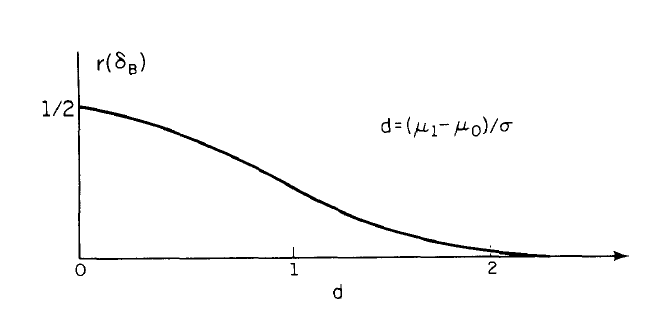
\includegraphics[width=0.6\linewidth]{Figures/Gauss_Bayes}
\caption{Bayes risk in location testing with Gaussian error}
\label{fig:bayeserror}
\end{figure}\\\\
\textbf{Minimax rule}\\\\
We know that $V(\pi_0)=r(\pi_0,\delta_{\pi_{0}})$. Now $V(0)=C_{11}$ and $V(1)=C_{00}$, regardless of the cost structure as it only depends on prior and hence the least favourable prior $\pi_{L}$ is in the interior (0,1) in this case. Moreover, since equation \ref{eq:33} is a differentiable function of $\pi_{0}$, randomization is unnecessary, and $\pi_{L}$ can be found by setting $R_{0}(\delta_{\pi_{L}})=R_{1}(\delta_{\pi_{L}})$.[That randomization is unnecessary also follows by noting that $P_{0}(L(Y)=\tau)=P_{1}(L(Y)=\tau)=0$ for any $\tau$ since $L(Y)$ is a continuous random variable.] The prior $\pi_{0}$ enters $R_{0}(\delta_{\pi_{0}})$ and $R_{1}(\delta_{\pi_{0}})$ only through $\tau'$, so an equalizer rule is found by solving
\begin{equation}
1-\Phi\Bigl(\frac{\tau'-\mu_0}{\sigma}\Bigr)=\Phi\Bigl(\frac{\tau'-\mu_1}{\sigma}\Bigr)
\end{equation}
By even symmetry property og Gaussian distribution function we have
\begin{equation}
\frac{\tau'-\mu_0}{\sigma}=\frac{\mu_1-\tau'}{\sigma}
\end{equation}
The unique solution is given by the following, which is also clear from the figure \ref{fig:minimaxerror}
\begin{equation}
\tau'=\frac{\mu_{0}+\mu_{1}}{2}\label{eq: 39}
\end{equation}
So the minimax decision rule is $\delta_{\pi_L}=\mathds{1}_{\{ y\geq\frac{\mu_{0}+\mu_{1}}{2}\}}$
from \ref{eq: 39} it follows that the least favourable prior $\pi_L=\frac{1}{2}$ so the minimax risk is
\begin{equation}
V\Bigl(\frac{1}{2}\bigr)=1-\Phi\Bigl(\frac{\mu_1-\mu_0}{2\sigma}\Bigr)
\end{equation}
\begin{figure}[h]
\centering
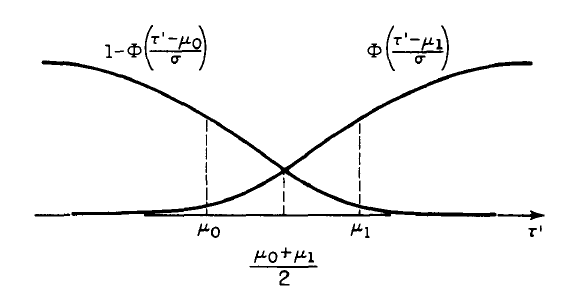
\includegraphics[width=0.6\linewidth]{Figures/Gauss_Minimax}
\caption{Conditional risk for location testing with Gaussian error and uniform cost}
\label{fig:minimaxerror}
\end{figure}\\
\textbf{Neyman Pearson rule}\\\\
Here we have
\begin{align}
P_F(\tilde{\delta}_{NP})&=P_0\{L(Y)>\eta\}\nonumber\\
					  &=P_0\{Y>L^{-1}(\eta)\}\nonumber\\
					  &=1-\Phi\Bigl(\frac{\eta'-\mu_0}{\sigma}\Bigr)\label{eq:29}
\end{align}
 where $\eta'=\frac{\mu_{0}+\mu_{1}}{2}+\frac{\sigma^2}{\mu_1-\mu_0}\log\eta$, and the curve of equation \ref{eq:29} is shown in figure \ref{fig:neymanerror}. Note that any value of $\alpha$ can be achieved by exactly choosing
\begin{equation}
\eta_0'=\mu_{0}+\sigma\Phi^{-1}(1-\alpha)
\end{equation}
where $\Phi^{-1}$ is the inverse function of $\Phi$. Since $P(Y=\eta_0)=0$ the randomization can be chosen arbitrarily say $\gamma_0=1$. An $\alpha$ level Neyman-Pearson test for this case is given by
\begin{align}
\tilde{\delta}_{NP}&=
				   \begin{cases}\nonumber 
				   1-y\geq\eta_0\label{eq:46} \\
				   0-y<\eta_0\\
				   \end{cases}\\
				&=\mathds{1}_{\{ y\geq\eta_0 \}}
\end{align}
\begin{figure}[h]
\centering
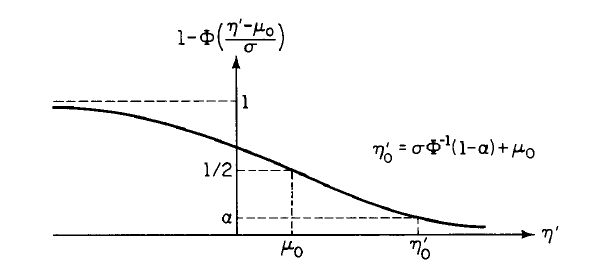
\includegraphics[width=0.7\linewidth]{Figures/Gauss_Neyman}
\caption{Illustration of threshold $\eta'_{0}$ for Neyman-Pearson testing of location with Gaussian error}
\label{fig:neymanerror}
\end{figure}
The detection probability of $\tilde{\delta}_{NP}$ is given by
\begin{align}
P_D(\tilde{\delta}_{NP})&=P_1\{Y\geq\eta_0\})\nonumber\\
					  &=1-\Phi(\frac{\eta'-\mu_1}{\sigma})\label{eq:49}\nonumber\\
					  &=1-\Phi(\Phi^{-1}(1-\alpha)-d)
\end{align}\\
Where $d=\frac{\mu_{1}-\mu_{0}}{\sigma}$ as appeared previously in case of Bayes hypothesis testing. For fixed $\alpha$, equation \ref{eq:49} gives the detection probability as a function of \textit{d} for the test of . This relationship is sometimes known as the power function for the test of equation \ref{eq:49}. A plot of this relationship is shown in figure \ref{fig:Power}. Equation \ref{eq:46} also gives the detection probability as a function of the false-alarm probability for fixed \textit{d}. Again borrowing from radar terminology, a parametric plot of this relationship is called the \textit{receiver operating characteristics}(ROCs). The ROCs for the test of \ref{eq:46} are shown in figure \ref{fig:ROC}.
\begin{figure}[h]
\centering
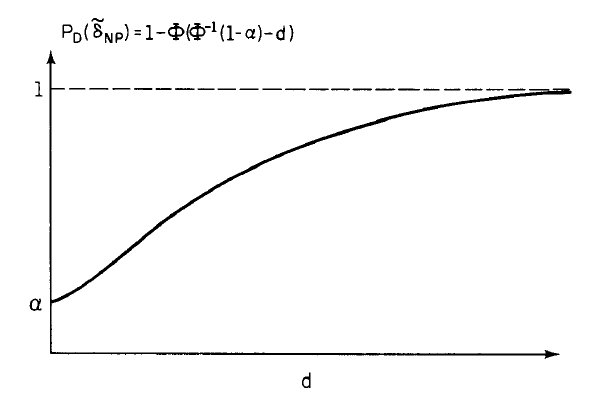
\includegraphics[width=0.5\linewidth]{Figures/Power}
\caption{Power function for Neyman-Pearson testing for location testing with Gaussian error}
\label{fig:Power}
\end{figure}
\begin{figure}[h]
\centering
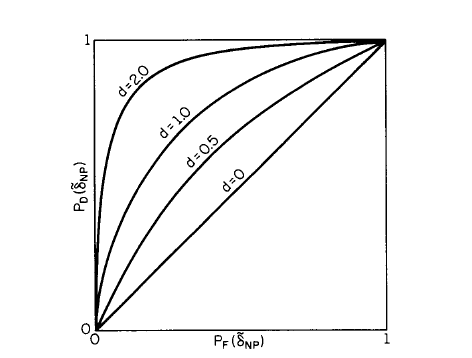
\includegraphics[width=0.5\linewidth]{Figures/ROC}
\caption{ROC curve for Neyman-Pearson testing for location testing with Gaussian error}
\label{fig:ROC}
\end{figure}
\end{exmp}

\begin{exmp}[The Binary Channel]
On a Binary Communication Channel a binary digit is to be transmitted. Our observation Y is the output of the channel, which can also be either zero or one.Due to channel noise a transmitted ``zero" is received as a ``one" with probability $\lambda_0$ and as a ``zero" with probability (1 - $\lambda_0$), where $0 \leq \lambda_0 \leq 1$. Similarly, a transmitted ``one" is received as a ``zero" with probability $\lambda_1$ and as a ``one" with probability (1- $\lambda_1$). Thus, the observation Y does not always represent which among the ``zero" or a ``one" transmitted. So we need to develop a technique to optimally detect the transmitted digit.
\begin{figure}[h]
\centering
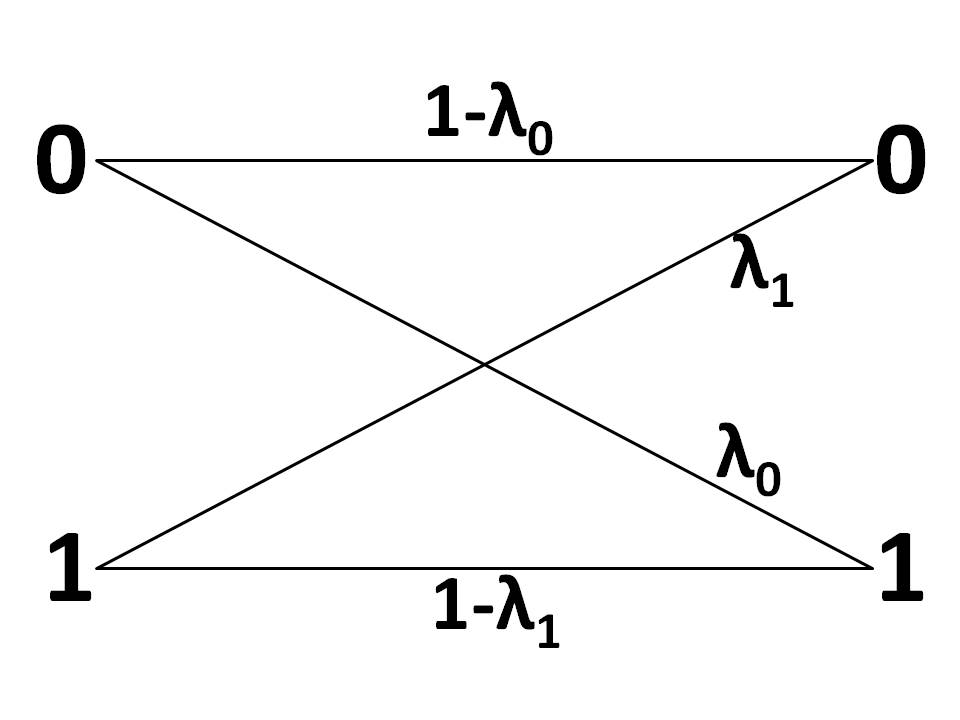
\includegraphics[width=0.6\linewidth]{Figures/bsc1}
\caption{The binary channel}
\label{fig:binary}
\end{figure}\\
This situation is clearly a Hypothesis Testing problem with the two hypothesis $ H_0~ and~ H_1 $ depicted as transmission of a ``zero" and transmission of a ``one" respectively. The observation set is $\Gamma$ \{0,1\}. The received signal $Y \in \Gamma$  will have a probability density function as follows:\\
\begin{eqnarray}
Y_{0}~\sim~\left( 1-\lambda_{0}\right) ~if~H_0~is~transmitted\\
Y_{1}~\sim~\left( 1-\lambda_{1}\right)~if~H_1~is~transmitted \end{eqnarray}
and the observation Y has densities (i.e., probability mass functions):
\begin{equation}
p_{j}\left( y\right) = \lambda_{j} ,~if~ y\neq j,
\end{equation}
\begin{equation}
p_{j}\left( y\right) = \left( 1-\lambda_{j}\right),~if~ y=j
\end{equation}
for $j \in \{0,1\}$.
\\\\
\textbf{Bayesian Hypothesis testing}\\\\
The likelihood ratio will then be given by \\

\begin{eqnarray}
L(y) = \frac{p_1(y)}{p_0(y)} =
								\begin{cases}
								\frac{\lambda_1}{1-\lambda_0} ~~~~~~~if~ y=0 \\
								\frac{1-\lambda_1}{\lambda_0} ~~~~~~~if~ y=1\\
								\end{cases} 
\end{eqnarray}
For certain threshold $\tau$ the decision rule is
\begin{eqnarray}
\delta_{B}(y)= 
				\begin{cases} \mathds{1}_{\bigl\{\frac{\lambda_1}{1-\lambda_0}\geq\tau\bigr\}} ~~~~~~~if~ y=0~~[we~write~it~as~ \mathds{1}_{A}~(event~A)]\\
				\mathds{1}_{\bigl\{\frac{1-\lambda_1}{\lambda_0}\geq\tau\bigr\}} ~~~~~~~if~ y=1~~[we~write~it~as ~\mathds{1}_{B}~(event~B)]\\
				\end{cases}
\end{eqnarray}
Then the conditional risks are given by the following equations
\begin{align}
R_{0}(\delta_{\pi_{0}})&=P_{0}(\Gamma_{1})\nonumber\\
					   &=\lambda_{0}\mathds{1}_{B}+(1-\lambda_{0})\mathds{1}_{A}\\
R_{1}(\delta_{\pi_{0}})&=P_{1}(\Gamma_{0})\nonumber\\
					   &=(1-\lambda_{1})\mathds{1}_{B^{c}}+\lambda_{1}\mathds{1}_{A^{c}}
\end{align}
The unconditional risk is given by
\begin{align}
r(\pi_{0},\delta_{\pi_{0}})&=\pi_{0}\lambda_{0}\mathds{1}_{B}+\pi_{0}(1-\lambda_{0})\mathds{1}_{A}+(1-\pi_{0})(1-\lambda_{1})(1-\mathds{1}_{B})+\nonumber\\
						   &~~~~(1-\pi_{0})\lambda_{1}(1-\mathds{1}_{A})\nonumber\\
						   &=(1-\pi_{0})(1-\lambda_{1})-{\{(1-\pi_{0})(1-\lambda_{1})-\pi_{0}\lambda_{0}\}}\mathds{1}_{B}+\nonumber\\
						   &~~~~(1-\pi_{0})\lambda_{1}-{\{(1-\pi_{0})\lambda_{1}-\pi_{0}(1-\lambda_{0})\}}\mathds{1}_{A}
\end{align}
To proceed further we need the following 
\begin{align}
A&=\Bigl\{\frac{\lambda_{1}}{1-\lambda_{0}}\geq\dfrac{\pi_{0}}{1-\pi_{0}}\Bigr\}~means~event~A~is~true\nonumber\\
B&=\Bigl\{\frac{1-\lambda_{1}}{\lambda_{0}}\geq\dfrac{\pi_{0}}{1-\pi_{0}}\Bigr\}~means~event~B~is~true\nonumber
\end{align}
We know that
\begin{align}
f(a)&=a\mathds{1}_{\{a\geq0\}}\nonumber\\
	&=(a)_{+}\nonumber\\
	&=max\{a,0\}
\end{align}
So unconditional risk becomes
\begin{align}
r(\pi_{0},\delta_{\pi_{0}})&=(1-\pi_{0})(1-\lambda_{1})-{\Bigl\{(1-\pi_{0})(1-\lambda_{1})-\pi_{0}\lambda_{0}\Bigr\}}_{+}+\nonumber\\
									  &~~~~(1-\pi_{0})\lambda_{1}-{\Bigl\{(1-\pi_{0})\lambda_{1}-\pi_{0}(1-\lambda_{0})\Bigr\}}_{+}\nonumber\\
									  &=\min{\Bigl\{(1-\pi_{0})(1-\lambda_{1}),\pi_{0}\lambda_{0}\Bigr\}}+\min{\Bigl\{(1-\pi_{0})\lambda_{1},\pi_{0}(1-\lambda_{0})\Bigr\}}\label{eq:70}
\end{align}
Again if $\pi_{0}=1-\pi_{0}$, $\therefore~\pi_{0}=\frac{1}{2}$.
\begin{equation}
\therefore r\Bigl(\frac{1}{2},\delta_{\frac{1}{2}}\Bigr)= min{\Bigl\{(1-\lambda_{1}),\lambda_{0}\Bigr\}}+min{\Bigl\{\lambda_{1},(1-\lambda_{0})\Bigr\}}
\end{equation}
\\\\
\textbf{Minimax rule}\\\\
From the equation \ref{eq:70} there is only two possibilities as follows
\begin{align}
\pi_{0}(1-\lambda_{0})&\leq\lambda_{1}(1-\pi_{0})\\
\pi_{0}\lambda_{0}&\leq(1-\pi_{0})(1-\lambda_{1})
\end{align}
Now we define the quantity $\underline{\pi}~and~\overline{\pi}$ 
\begin{eqnarray}
\underline{\pi}=\min\Bigl\{\frac{\lambda_{1}}{1-\lambda_{0}+\lambda_{1}},\frac{1-\lambda_{1}}{1-\lambda_{1}+\lambda_{0}}\Bigr\}\nonumber\\
\overline{\pi}=\max\Bigl\{\frac{\lambda_{1}}{1-\lambda_{0}+\lambda_{1}},\frac{1-\lambda_{1}}{1-\lambda_{1}+\lambda_{0}}\Bigr\}\nonumber
\end{eqnarray}
The unconditional risk can be written as
\begin{equation}
r(\pi_0,\delta_{\pi_0})= \begin{cases} \pi_0~~ If~~ \pi_0\leq\underline{\pi}\\
 						1-\pi_0 ~~If ~~\pi_0\geq\overline{\pi}  \\
  						\underline{\pi}+\Bigl(\frac{1-\overline{\pi}-\underline{\pi}}{\overline{\pi}-\underline{\pi}}\Bigr)
(\pi_0-\underline{\pi})~~If ~~\underline{\pi}<\pi_0<\overline{\pi}
\end{cases}
\end{equation}

Say $c=\Bigl(\frac{1-\overline{\pi}-\underline{\pi}}{\overline{\pi}-\underline{\pi}}\Bigr)$, Then if $c>0$ then $\pi_L=\overline{\pi}$ . If $c<0$ then $\pi_L=\underline{\pi}$. And if $c=0$ then any q will work, where q is the probability of picking ``one" at the threshold. So pick a randomized rule at the threshold.\\
Now recall that
\begin{equation}
q= \frac{V'(\pi^+_L)}{V'(\pi^+_L)-V'(\pi^-_L)}
\end{equation}
Where $V'(\pi_0)$ is the derivative of V with respect to $\pi_0$. Now assume $c>0$ then $q=\frac{-1}{-1-c}=\frac{1}{1+c}$, which is clear from the figure \ref{fig:binaryminimax}\\
\\
\begin{figure}[h!]
\centering
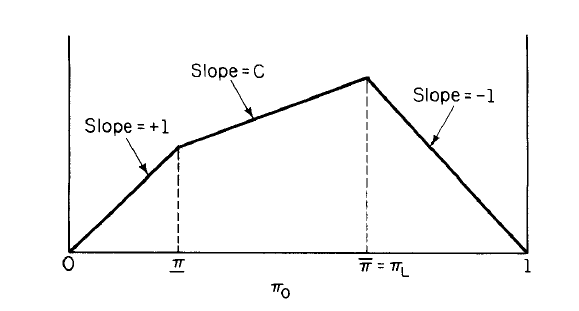
\includegraphics[width=0.6\linewidth]{Figures/Binary_Minimax}
\caption{$V(\pi_0)$ for the binary channel}
\label{fig:binaryminimax}
\end{figure}
If $\pi_L=\overline{\pi}$ then $V(\overline{\pi})=1-\overline{\pi}>\underline{\pi}$. And if $\pi_L=\underline{\pi}$ then $V(\underline{\pi})=\underline{\pi}>1-\overline{\pi}$\\
\begin{equation}
\therefore V(\pi_L)= max{\{\underline{\pi},1-\overline{\pi}}\}
\end{equation}
Now the decision rule is
\begin{equation}
\delta_{\pi_0}(y)=\begin{cases}0~~,\forall y ~if~ \pi_0\geq\overline{\pi}\\
				1~~,\forall y~ if~ \pi_0\leq\underline{\pi}\\
				\end{cases}\\
\end{equation}
And if $\pi_0\in\{\underline{\pi},\overline{\pi}\}$
\begin{align}
\delta_{\pi_0}(0)&=\mathds{1}_{A^{c}}\\
\delta_{\pi_0}(1)&=\mathds{1}_{B}
\end{align}
Say $c>0$ the by inspection we have $\pi_L=\overline{\pi}$ and $\delta^{+}_{\pi_L}(y)=0~,~\Gamma_{1}^{+}=\phi$\\
So the decision rule is
\begin{equation}
\delta_{\pi_0}(y)= \begin{cases}
y ~~~~~~~~~~if ~\frac{1-\lambda_1}{1-\lambda_0-\lambda_1}\geq\pi_0>\frac{\lambda_1}{1-\lambda_0-\lambda_1}\\
1-y ~~~~~if ~\frac{\lambda_1}{1-\lambda_0-\lambda_1}\geq\pi_0>\frac{1-\lambda_1}{1-\lambda_0-\lambda_1}
\end{cases}
\end{equation}


\end{exmp}

\end{document}
